\section{Data}
\label{sec:data}
\textit{``The most satisfactory sampling design for structural analysis is a saturation sample of the entire universe or population; 
however, this alternative is clearly not feasible for large social structures'' 
}
\begin{flushright}
--- M.P. Allen, 1974
\end{flushright}

\subsection{Data description}
The data from this project was extracted from Orbis.
Orbis contains standardized information from 200 million firms and 100 million people. 
The firm data includes economic indicators (such as turnover, employee number, profit ratios or economic activity (standardized using NACE rev. 2)),
as well as 90 million ownership ties.
The directors data includes biographic information (such as name, education, nationality or gender), 
as well as 151 million position information.
Importantly, a person sitting on the board of two companies creates a connection between the firms (interlocks).
Since directors can sit on more than one boards, 
the database has more than 1,000 million interlocks.

The concept of interlocking directorates is related to the corporate elite, part of the power elite. 
Mills~\cite{mills1957} defined the power elite as \textit{``those political, economic, and military circles, which as an intricate set of overlapping small but dominant groups share decisions having at least national consequences. Insofar as national events are decided, the power elite are those who decide them''}~\citep{mills1957}. 
Moreover, Mills determined that there is an `inner core' of the power elite involving individuals that are able to move from one seat of institutional power to another. 
In the context of corporations, this inner core corresponds to the corporate elite. 
A strength of using the concept of interlocking directorates as opposed to corporate elites is that we do not assume a priori characteristics of the elite. 
Corporate elites on the interlock network are the actors with high centralities values, as measured by network algorithms.

The first step of the project consists on downloading, structuring and storing the data (months 1-4), quantifying the quality of the data (months 4-7) and assessing the effect on the results (months 8-10). For brevity we will skip most the details of the quality assessment. Figure ~\ref{fig:qual}A compares the number of companies in Orbis with the OECD. We can see that the quality is extremely good for large companies, but relatively bad for small companies. However, the companies in Figure ~\ref{fig:qual}A are those with available revenue and employment information (~60 million instead of 200). Thus, we have most companies in the database, but without financial information. 

We developed a two-step approach to assess the quality of the data. In the first step, we developed interactive visualizations to rapidly explore the data (see \url{https://github.com/uvacorpnet}). The results showed that richer countries (measured by GDP per capita) have larger companies and better data completeness. The visualizations also showed that the observed average revenue for the companies in a country depends on the completeness. Those with higher completeness include also small companies, decreasing the revenue of the `average' company. In the second step, we characterized the data and extrapolate the quality to other countries. The distributions of revenue for a country follow a lognormal distribution, thus can be defined using two parameters (loc and scale). Moreover, the scale is fixed for all countries and the loc can be estimated using macro-economic indicators. This allows to quantify the type of missing companies (Fig. ~\ref{fig:qual}B). In the next month we will assess the effect of completeness in network measures. 
This assessment will determine to what extent our results are generalizable. 

\begin{figure}
\begin{center}
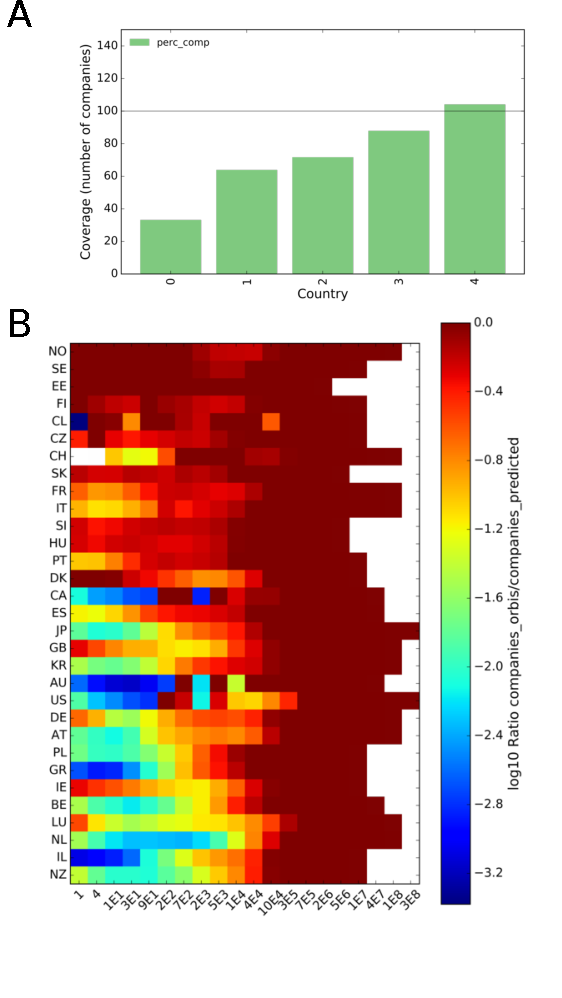
\includegraphics[width=.5\textwidth]{qual.pdf}
\caption{Data quality.}
\label{fig:qual}
\end{center}
\end{figure}

\subsection{Data bias}
We position ourselves very far from the data. 
Given the scope of the project (study the role of interlocks globally) this is the only viable solution.  
However, the validity of the measurements is still high because we focus on physical phenomena 
-- the distribution of companies in a city and the presence of interlocks between companies.
In order to operationalize the concept of city, 
we understand city as a geographic region with high density of settlements.
To find regions with high density of settlements 
we use the \textit{MeanShift} algorithm~\citep{fukunaga1975}.
This allow us to automatically merge Boston and Cambridge, New York City and Brooklyn, or Amsterdam and Amstelveen.



We will next talk about completeness (how much of the data we have), 
bias (is our sample a random sample), 
and accuracy (is the data we have true). 

\textit{Company data}
1. Bias and completeness: 
We have assessed the bias and completeness of the data (Fig. ~\ref{fig:qual}B). 
In general, Scandinavian countries have the highest quality (very complete and fairly unbiased), 
while poor countries only have information about their biggest companies.
We can now use our method to reconstruct missing data and assess the effect of including it. 
We expect the effect to be small since small companies are not usually connected in the network -- for example the owner of a small shop is not likely to sit in the board of directors of any company.

2.  Accuracy: 
We have checked the accuracy of a random sample and the information in the database is almost always correct. 
However, there are some problems in this area. 
Some information providers send their data faster than others, which makes the information of some countries be outdated up to one year. 
Moreover, large company generally are required to fill consolidated accounts, 
including in their reports the profits, employees and other economics of their subsidiaries. 
Because we also have information about the subsidiaries in our database, 
the profits of the subsidiaries are registered twice.
However, because we have information about the subsidiaries,
we can unconsolidate the accounts.
Figure ~\ref{fig:qual} are based on the unconsolidated results.

\textit{Directors data}
Missing actors in social networks produce less bias in the network than missing companies~\citep{Kossinets2006}.
This is important since directors data is harder to check.

1. Bias and completeness: 
Based on manual inspection of a small sample of the data we found that some directors from small companies are missing. 
However, we can create confidence intervals by imputing missing (rewiring the network)

2.  Accuracy: 
We found that large companies have extra directors that have already left the company. 
However, we can create confidence intervals by imputing missing (rewiring the network)
Moreover, the type of position of directors in some countries is unspecified, 
meaning that we do not know if the person is an administrative (e.g. secretary, lawyer, etc) or a director.
However, we can remove administrative ties by using the ownership database. 
If a director has positions in a shareholder and a wholly owned subsidiary then we can filter that tie. 
A consideration in this approach is that two subsidiaries that are wholly owned by company A may not have any ownership relationship between them, 
but they are still the same corporation. 
We can correct this by deleting all ties within the same corporate structure.


A final consideration is in the concept of interlocks. 
We want to measure relationships between companies. 
However it is not clear that formal interlocks -- those occurring by people sitting together on boards -- 
are more important than interlocks created by directors being part of the same social clubs or the same families. 
By restricting ourselves to formal interlocks we may be missing an important part of the corporate network. 
However, we expect to capture a significant part of the relations between companies.

 